\documentclass{report}
\usepackage{fullpage}
\usepackage[backend=biber]{biblatex} 
\addbibresource{bibliography.bib}
\usepackage{hyperref}
\hypersetup{
	pdfborderstyle={/S/U/W 1}
}

\usepackage{amsmath}
\usepackage{amssymb}
\usepackage{float}
\usepackage{tikz}
\usepackage{pgfplots}
\usepackage{xcolor}

\usepackage{graphicx}
\graphicspath{./figures}

\begin{document}
	\title{CAB420 Project Report \\ \large{Movie Rating Prediction}}
	\author{
		Jarrod Williams\\
		\texttt{n9722068}\\
		\emph{\dots\%}
		\and 
		Caleb Geizer\\
		\texttt{n9488243}\\
		\emph{\dots\%}
		\and
		Alex Barnier\\
		\texttt{n9448551}\\
		\emph{\dots\%}
		\and	
		Madeline Miller\\
		\texttt{n9342401}\\
		\emph{\dots\%}
	}
	\date{June, 2018}
	\maketitle
	
	\chapter{Introduction}
	\section{Motivations}
	As businesses strive to increase user interaction with their products and services, recommendation systems have seen widespread adoption. One such business is Netflix, arguably the largest platform for watching and rating movies, who uses recommendation systems to provide its users with movies it believes are relevant to their tastes. This is achieved by training its recommender system on millions of user reviews. In 2009 Netflix issued a challenge to the community to design a recommendation algorithm that was better than their algorithm at the time. This challenge, called the ‘Netflix Prize’, aimed to create an algorithm with a Root-Mean-Squared-Error (RMSE) of 90\% of their existing one or better.
	
	The motivation for this project was to develop our own solution for this challenge and help better the performance of movie recommendation algorithms. The Netflix Prize winner was announced in 2011 and had a RMSE of 0.8567 \autocite{NeflixLeader}. It is our goal to build a recommender system with a RMSE within the top ten teams, (i.e. RMSE < 0.8624).
	
	\section{Related Work}
	A common approach to creating a recommendation system using this data is using a k-means clustering algorithm to group different users together based on their preferences. This method is used to create larger sample sizes for ratings by treating one cluster as a single user \autocite{CS229}.
	These clusters can then be used in conjunction with a classifier, like naive bayes, to create the final recommendation system. By using a naive bayes classifier features like the genre of specific movies or other metadata can be added as a feature to create more refined probabilities. This can also be applied to a multi-class logistic regression classifier \autocite{Bystrom}, where certain features can be given weights, which would allow for place importance on certain genres or directors (if present).
	
	
	How do we extend these approaches?
	The objectives of this report are to extend the existing approaches put forward by Huang and Bystr\"om to get a classifier close to, or less than the Netflix Prize qualification RMSE of 0.8572 \autocite{NeflixRules}.

	
	\chapter{Experiment}
	\section{MovieLens Data}
	\subsection{The Dataset}
	The MovieLens data set consists of approximately 100,000 user ratings for films of various genres and release dates. Each rating is out of 5, representing the ‘star-ratings’ users have assigned to the film. Partial star ratings (e.g. 2.5 stars) are also given, allowing for a total of 10 possible ratings (0.5 - 5 stars). Included with each rating is the film id which links to another table containing the film’s title, genre(s) and release date. As one of the features of the MovieLens website is the ability to add tags to films, the dataset also contains a list of user-defined tags for the movies. Finally, there is a table that links the MovieLens id’s for films to their corresponding id on other community sites like IMDb (Internet Movie Database) and TMDb (The Movie Database). Combined, these tables represent 9125 movies, 100004 user-ratings from 671 users and 1296 custom tags from 61 users.
	\subsection{Pre-processing}
	As this dataset was pre-configured for academic studies, it contained no invalid data (missing values, out-of-range values, etc). Preprocessing then was limited to selecting the target variable, rating, and relevant features userId, movieId and genre. Column headers were also extracted and panda dataframes were constructed to store this data. As multiple genres could be assigned to a single movie, multiple rows in the dataset contain the same userId and movieId with a different genre assigned to it. Finally, the data was split into four 75/25\% train-test splits using the Kfold function, part of the sklearn library.
	\subsection{Exploration of Data}
	Using the preprocessed data, a normalised heapmat of review scores can be generated, giving us insights into our training data [\autoref{fig:heatmap}]. 
	\begin{figure}
		\centering
		\includegraphics[width=\textwidth]{./figures/normalised_heatmap.png}
		\label{fig:heatmap}
		\caption{Normalised Heatmap of User Ratings}
	\end{figure}
	\section{Methedology}
	Three classification algorithms were used for this project: SVM, Random Forest and Gradient Boosting. For all algorithms, the target variable was set to rating with the \emph{userId}, \emph{movieId} and \emph{genre} features used for training and prediction.
	\subsection{SVM Classifier}
	Support Vector Machines (SVM) are a robust and accurate machine learning algorithm designed for classification problems. Originally designed for binary classification, modern SVMs are capable of multiclass classification, regression, ranking and time series prediction \autocite{KarlPersson}. Support vector machines work by separating data using a linear line or hyperplane; separating nonlinear data requires the use of kernel tricks.
	For this project an SVM from the sklearn library was trained, using a linear kernel. Due to the size of the dataset, the execution time for this classifier exceeded 36 hours, at which time training was terminated. As a result, we were unable to produce a trained model and conduct testing on it.
	\subsection{Random Forest Classifier}
	Random Forest classifiers construct a collection of decision trees for each feature and average the result of these trees to improve their accuracy. 	
	The Random Forest classifier used in this report has three important hyperparameters that were tweaked to increased the predictive power of the algorithm:
	
	\begin{itemize}
		\item {\textbf{n\_estimators}: The total number of trees the classifier builds prior to taking the averages of predictions. 
		\subitem {Values tested: [10, 50, 100, 250, 500]}
		\subitem {Optimal value found: 500}}
		\item {\textbf{min\_samples\_split}: The minimum number of samples required to split a node.
		\subitem Values tested: [3, 7 , 15]
		\subitem{ Optimal value found: 7}}
		\item {\textbf{min\_samples\_leaf}: The minimum number of leafs required to split an internal node.
		\subitem {Values tested: [3, 7, 15]}
		\subitem {Optimal value found: 15}}		
	\end{itemize}
	
	\subsection{Gradient Boosting Classifier}
	A machine learning technique that produces an improved algorithm from a collection or ensemble of weaker learner models, in this case decision trees. 
	\begin{itemize}
		\item \textbf{n\_estimators}: Total number of boosting stages to perform.  
		\subitem Values tested: [100, 500, 1000]
		\subitem Optimal value found: 500
		\item \textbf{min\_samples\_split}: The minimum number of samples required to split a node.
		\subitem Values tested: [7 , 15]
		\subitem Optimal value found: 7
		\item \textbf{min\_samples\_leaf}: Minimum number of samples required in a terminal node or leaf. 
		\subitem Values tested: [7, 15]
		\subitem Optimal value found: 15	
		\item \textbf{max\_depth}: The maximum depth of the tree. 
		\subitem Values tested: [3, 10]	
		\subitem Optimal value found: 10
		
	\end{itemize}
	\section{Parameter Optimisation}
	In order to determine which algorithm and associated hyperparameters produced the most accurate model, parameter optimisation was implemented. This involved testing the root mean square error of a set of possible parameters for each algorithm. By iterating through all of the possible combinations, and finding the lowest error, we were able to determine which was the best set of parameters for usage in our model.	
	Using parameter optimisation is not without its downsides however, as this can introduce overfitting to the test data. In order to avoid this, cross validation on 4 different splits of data was implemented and tested against the mean of the resulting root mean squared error. This allows us to be sure that the parameters work for a wider range of test data than just a single set.
	
	\chapter{Results}
	\section{Comparison and Discussion}
	\begin{table}[H]
		\centering
	\begin{tabular}{ccc}
		\hline
		Algorithm & RMSE & \% Improvement\\
		\hline
		K-Means w/ Logistic \autocite{Bystrom} & 0.884 & 7.19	\\
		K-Means w/ Na\"ive Bayes \autocite{CS229} & 1.28 & -32.72\\
		Netflix Prize Winner & 0.8567 & 10.06\\
		\hline
	\end{tabular}
	\caption{Comparision of Existing Methods}
	\label{tab:pastresults}
	\end{table}
	\begin{table}[H]
		\centering
		\begin{tabular}{ccc}
			\hline
			Algorithm & RMSE & \% Improvement\\
			\hline
			SVM & $\infty$ & \dots	\\
			Random Forest & 1.091 & \dots\\
			Gradient Boosting & 0.8626 & 8.99\\
			\hline
		\end{tabular}
	\caption{Comparison of Our Results}
	\label{tab:ourresults}
	\end{table}
	The results seen in \autoref{tab:pastresults} and \autoref{tab:ourresults} show that of all approaches attempted in this report, the Gradient Boosting classifier provided the best results with an average RMSE value of 0.8626, ~9\% better than the Netflix baseline. It’s best RMSE measured was 0.8598, coming just 0.31\% shy of the Netflix Prize Winner’s RSME of 0.8567.
	
	The Random Forest classifier did not fare as well however with its RMSE of 1.091 being 13.85\% worse than the Netflix Baseline RMSE. The classifier did still produce a model however, a feat the SVM algorithm was unable to achieve after 36 hours of training. The Random Forest was also the fastest model to train, beating both the Gradient Boosting and SVM models in training time.
	
%	\begin{figure}[H]
%		\centering
%		\begin{tikzpicture}
%			\begin{axis}[xbar stacked,
%			symbolic y coords={SVM,Random Forest,Gradient Boosting},
%			ytick=data]
%				\addplot[xbar,fill=blue] coordinates {
%					(0,SVM)
%					(1.091,Random Forest)
%					(0.8,Gradient Boosting)
%				};
%				%\addplot[no marks] coordinates {(0.9525,SVM) (0.9525,Gradient Boosting)};
%				\draw[ultra thin, red] (axis cs:0.9525,SVM) -- (axis cs:0.9525,{Gradient Boosting}) node[pos=0.03, below] {Cinematch};
%			\end{axis}
%		\end{tikzpicture}
%		\caption{Chart of Our Classifiers in Relation to Cinematch Baseline}
%		\label{fig:graphofours}
%	\end{figure}
	
	\begin{figure}[H]
		\centering
		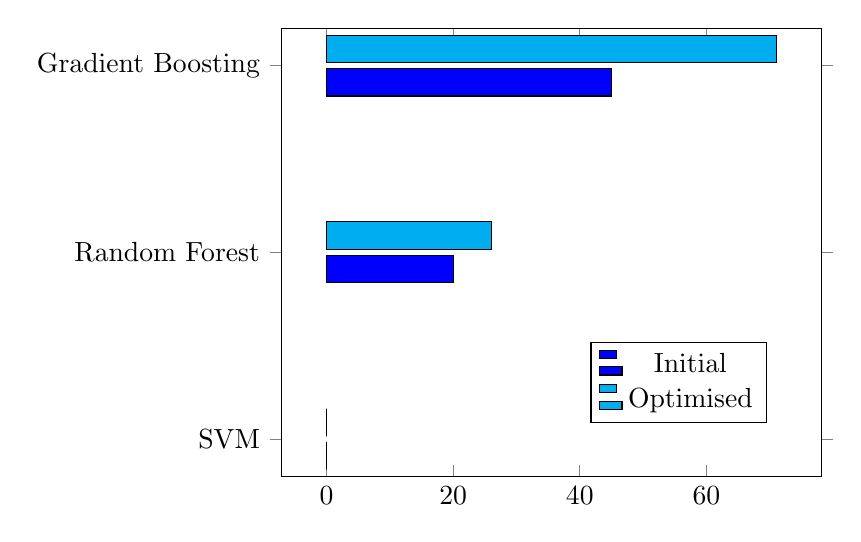
\begin{tikzpicture}
			\begin{axis}[xbar,
						symbolic y coords={SVM,Random Forest,Gradient Boosting},
						ytick=data,
						legend style = {at={(0.9,0.3)}}]
			\addplot[xbar,fill=blue] coordinates {
					(0,SVM)
					(20,Random Forest)
					(45,Gradient Boosting)
			};
			\addlegendentry{Initial};
			\addplot[xbar,fill=cyan] coordinates {
				(0,SVM)
				(26,Random Forest)
				(71,Gradient Boosting)
			};
			\addlegendentry{Optimised};
			\end{axis}
		\end{tikzpicture}
		\caption{Chart of Our Classifier Accuracy}
		\label{fig:graphofours}
	\end{figure}
	
	As seen in \autoref{fig:graphofours}, parameter optimisation provided a large accuracy boost to both the Random Forest and Gradient Boosting algorithms. With an initial accuracy of 20\%, the optimised Random Forest model proved 60\% more accurate with a final accuracy of ~33\%. This is a little less than the unoptimised Gradient Boosting model which has an initial accuracy of 45\%. Post parameter optimisation, this model was 71\% accurate, an increase of ~63\% from it’s initial model.
	
	\chapter{Conclusion}
	The experiments conducted in this report show that the Gradient Boosting classifier completes the objective of developing an effective movie rating prediction algorithm. The algorithm’s Root-Mean-Squared-Error of 0.8598 places it within the top 10 algorithms in the Netflix Prize contest, achieving the goal outlined in the introduction. Other algorithms tested, the Random Forest and SVM classifiers were unable to achieve this goal however.
	
	A shortcoming of our approach was that the dataset used was designed to easily develop these types of recommendation algorithms. Therefore, there was no invalid or misclassified data in the dataset that might reduce the accuracy of the trained models.
	
	Future investigations for the proposed approach would dive into testing the accuracy of the algorithm when it has fewer amounts of data points per user and using more features for training the models. Such proposed investigations include: 
	\begin{itemize}
		\item Training and testing the Gradient Boosted Classifier on a larger, more diverse dataset containing partial bad data.
		\item Including film release dates and user given tags as features and determining if the accuracy of the algorithm can be increased.
	\end{itemize}
	
	\newpage
	\printbibliography
	
\end{document}